% *****************************************************************************************************
% ****************************                 HW2                     ********************************
% *****************************************************************************************************

% =======================================================
% =======         HEADER FOR DOCUMENT        ============
% =======================================================
    
    % *********  SPECIFIC FOR THIS BOOK  ********
    \def\ProjectAuthorLink{https://github.com/CompilandoConocimiento}
    \def\ProjectNameLink{\ProjectAuthorLink/RandomProject}    
    

    % *********   DOCUMENT ITSELF   **************
    \documentclass[12pt, fleqn]{report}                             %Type of doc and size of font and left equations
    \usepackage[margin=1.2in]{geometry}                             %Margins and Geometry pacakge
    \usepackage{ifthen}                                             %Allow simple programming using if - then
    \usepackage[hidelinks]{hyperref}                                %Allow to create hiperlinks and Fuck Firefox
    \usepackage{pdfpages}                                           %Allow us 'import' PDF's
    \hypersetup{pageanchor=false}                                   %Solve 'double page 1' warnings in build :v
    \setlength{\parindent}{0pt}                                     %Eliminate ugly indentation
    \author{Oscar Andrés Rosas}                                     %Who I am

    % *********   LANGUAJE    *****************
    \usepackage[spanish]{babel}                                     %Please allow me to type in spanish
    \usepackage[utf8]{inputenc}                                     %Lets use UFT-8
    \usepackage[T1]{fontenc}                                        %Allow for better font support
    \usepackage{textcmds}                                           %Allow us to use quoutes
    \usepackage{changepage}                                         %Allow us to use identate paragraphs
    \usepackage{anyfontsize}                                        %All the sizes for fonts wiiiii!

    % *********   MATH AND HIS STYLE  *********
    \usepackage{ntheorem, amsmath, amssymb, amsfonts}               %All fucking math, I want all!
    \usepackage{mathrsfs, mathtools, empheq}                        %All fucking math, I want all!
    \usepackage{cancel}                                             %Negate symbol
    \usepackage{centernot}                                          %Allow me to negate a symbol
    \decimalpoint                                                   %Use decimal point

    % *********   GRAPHICS AND IMAGES *********
    \usepackage{graphicx}                                           %Allow to create graphics
    \usepackage{float}                                              %For images
    \usepackage{wrapfig}                                            %Allow to create images
    \graphicspath{ {Graphics/} }                                    %Where are the images :D

    % *********   LISTS AND TABLES ***********
    \usepackage{listings, listingsutf8}                             %We will be using code here
    \usepackage[inline]{enumitem}                                   %We will need to enumarate
    \usepackage{tasks}                                              %Horizontal lists
    \usepackage{longtable}                                          %Lets make tables awesome
    \usepackage{booktabs}                                           %Lets make tables awesome
    \usepackage{tabularx}                                           %Lets make tables awesome
    \usepackage{multirow}                                           %Lets make tables awesome
    \usepackage{multicol}                                           %Create multicolumns

    % *********   REMOVE SOME ERRORS **********
    \hbadness=10000                                                 %Ignore \vbox and \hbox warings
    \hfuzz=\maxdimen\newdimen\hfuzz                                 %Ignore \vbox and \hbox warings

    % *********   HEADERS AND FOOTERS ********
    \usepackage{fancyhdr}                                           %Lets make awesome headers/footers
    \pagestyle{fancy}                                               %Lets make awesome headers/footers
    \setlength{\headheight}{16pt}                                   %Top line
    \setlength{\parskip}{0.5em}                                     %Top line
    \renewcommand{\footrulewidth}{0.5pt}                            %Bottom line

    \lhead{                                                         %Left Header
        \hyperlink{section.\arabic{section}}                        %Make a link to the current chapter
        {\normalsize{\textsc{\nouppercase{\leftmark}}}}             %And fot it put the name
    }

    \rhead{                                                         %Right Header
        \hyperlink{section.\arabic{section}.\arabic{subsection}}    %Make a link to the current chapter
            {\footnotesize{\textsc{\nouppercase{\rightmark}}}}      %And fot it put the name
    }

    \rfoot{\textsc{\small{Oscar Andres Rosas Hernandez}}}     %This will always be a footer  
    \lfoot{\textsc{\small{Jorge Luís García De Santiago}}}     %This will always be a footer  

    
    
    
% =======================================================
% ===================   COMMANDS    =====================
% =======================================================

    % =========================================
    % =======   NEW ENVIRONMENTS   ============
    % =========================================
    \newenvironment{Indentation}[1][0.75em]                         %Use: \begin{Inde...}[Num]...\end{Inde...}
        {\begin{adjustwidth}{#1}{}}                                 %If you dont put nothing i will use 0.75 em
        {\end{adjustwidth}}                                         %This indentate a paragraph
    
    \newenvironment{SmallIndentation}[1][0.75em]                    %Use: The same that we upper one, just 
        {\begin{adjustwidth}{#1}{}\begin{footnotesize}}             %footnotesize size of letter by default
        {\end{footnotesize}\end{adjustwidth}}                       %that's it
    
    \def \Eq {equation}                                             %Stupid Visual studio error
    \newenvironment{MultiLineEquation}[1]                           %Use: To create MultiLine equations
        {\begin{\Eq}\begin{alignedat}{#1}}                          %Use: \begin{Multi..}{Num. de Columnas}
        {\end{alignedat}\end{\Eq}}                                  %And.. that's it!
    
    \newenvironment{MultiLineEquation*}[1]                          %Use: To create MultiLine equations
        {\begin{\Eq*}\begin{alignedat}{#1}}                         %Use: \begin{Multi..}{Num. de Columnas}
        {\end{alignedat}\end{\Eq*}}                                 %And.. that's it!

    \newenvironment{largeEq} {\begingroup \large}{\endgroup}        %Make eq bigger
    \newenvironment{LargeEq} {\begingroup \Large}{\endgroup}        %Make eq bigger
    \newenvironment{HugeEq} {\begingroup \Huge}{\endgroup}          %Make eq bigger!

    % =========================================
    % == GENERAL TEXT & SYMBOLS ENVIRONMENTS ==
    % =========================================
    
    % =====  TEXT  ======================
    \newcommand \Quote              {\qq}                           %Use: \Quote to use quotes
    \newcommand \Over               {\overline}                     %Use: \Bar to use just for short
    \newcommand \ForceNewLine       {$\Space$\\}                    %Use it in theorems for example
    \newcommand \ForceColumnBreak   {\vfill\null\columnbreak}       %Use only in multicols

    % =====  SPACES  ====================
    \DeclareMathOperator \Space     {\quad}                         %Use: \Space for a cool mega space
    \DeclareMathOperator \MegaSpace {\quad \quad}                   %Use: \MegaSpace for a cool mega mega space
    \DeclareMathOperator \MiniSpace {\;}                            %Use: \Space for a cool mini space
    
    % =====  MATH TEXT  =================
    \newcommand \Such           {\MiniSpace | \MiniSpace}           %Use: \Such like in sets
    \newcommand \Also           {\MiniSpace \text{y} \MiniSpace}    %Use: \Also so it's look cool
    \newcommand \Remember[1]    {\Space\text{\scriptsize{#1}}}      %Use: \Remember so it's look cool
    
    % =====  THEOREMS: IN SPANISH :0  ===
    \newtheorem{Theorem}        {Teorema}[section]                  %Use: \begin{Theorem}[Name]\label{Nombre}...
    \newtheorem{Corollary}      {Colorario}[Theorem]                %Use: \begin{Corollary}[Name]\label{Nombre}...
    \newtheorem{Lemma}[Theorem] {Lemma}                             %Use: \begin{Lemma}[Name]\label{Nombre}...
    \newtheorem{Definition}     {Definición}[section]               %Use: \begin{Definition}[Name]\label{Nombre}...
    \theoremstyle{break}                                            %THEOREMS START 1 SPACE AFTER Fuck!

    % =====  LOGIC  =====================
    \newcommand \lIff    {\leftrightarrow}                          %Use: \lIff for logic iff
    \newcommand \lEqual  {\MiniSpace \Leftrightarrow \MiniSpace}    %Use: \lEqual for a logic double arrow
    \newcommand \lInfire {\MiniSpace \Rightarrow \MiniSpace}        %Use: \lInfire for a logic infire
    \newcommand \lLongTo {\longrightarrow}                          %Use: \lLongTo for a long arrow
    \newcommand \lAnd    {\land}                                    %Use: \lAnd ^
    \newcommand \lOr     {\lor}                                     %Use: \lOr or symbol
    \newcommand \lNot    {\neg}                                     %Use: \lNot for negation

    % =====  FAMOUS SETS  ===============
    \DeclareMathOperator \Naturals     {\mathbb{N}}                 %Use: \Naturals por Notation
    \DeclareMathOperator \Primes       {\mathbb{P}}                 %Use: \Primes por Notation
    \DeclareMathOperator \Integers     {\mathbb{Z}}                 %Use: \Integers por Notation
    \DeclareMathOperator \Racionals    {\mathbb{Q}}                 %Use: \Racionals por Notation
    \DeclareMathOperator \Reals        {\mathbb{R}}                 %Use: \Reals por Notation
    \DeclareMathOperator \Complexs     {\mathbb{C}}                 %Use: \Complex por Notation
    \DeclareMathOperator \GenericField {\mathbb{F}}                 %Use: \GenericField por Notation
    \DeclareMathOperator \VectorSet    {\mathbb{V}}                 %Use: \VectorSet por Notation
    \DeclareMathOperator \SubVectorSet {\mathbb{W}}                 %Use: \SubVectorSet por Notation
    \DeclareMathOperator \Polynomials  {\mathbb{P}}                 %Use: \Polynomials por Notation
    \DeclareMathOperator \VectorSpace  {\VectorSet_{\GenericField}} %Use: \VectorSpace por Notation
    \DeclareMathOperator \LinealTransformation {\mathcal{T}}        %Use: \LinealTransformation for a cool T
    \DeclareMathOperator \LinTrans      {\mathcal{T}}               %Use: \LinTrans for a cool T
    \DeclareMathOperator \Laplace       {\mathcal{L}}               %Use: \LinTrans for a cool T

    % =====  CONTAINERS   ===============
    \newcommand{\Set}[1]            {\left\{ \; #1 \; \right\}}     %Use: \Set {Info} for INTELLIGENT space 
    \newcommand{\bigSet}[1]         {\big\{  \; #1 \; \big\}}       %Use: \bigSet  {Info} for space 
    \newcommand{\BigSet}[1]         {\Big\{  \; #1 \; \Big\}}       %Use: \BigSet  {Info} for space 
    \newcommand{\biggSet}[1]        {\bigg\{ \; #1 \; \bigg\}}      %Use: \biggSet {Info} for space 
    \newcommand{\BiggSet}[1]        {\Bigg\{ \; #1 \; \Bigg\}}      %Use: \BiggSet {Info} for space 
        
    \newcommand{\Wrap}[1]           {\left( #1 \right)}             %Use: \Wrap {Info} for INTELLIGENT space
    \newcommand{\bigWrap}[1]        {\big( \; #1 \; \big)}          %Use: \bigBrackets  {Info} for space 
    \newcommand{\BigWrap}[1]        {\Big( \; #1 \; \Big)}          %Use: \BigBrackets  {Info} for space 
    \newcommand{\biggWrap}[1]       {\bigg( \; #1 \; \bigg)}        %Use: \biggBrackets {Info} for space 
    \newcommand{\BiggWrap}[1]       {\Bigg( \; #1 \; \Bigg)}        %Use: \BiggBrackets {Info} for space 

    \newcommand{\Brackets}[1]       {\left[ #1 \right]}             %Use: \Brackets {Info} for INTELLIGENT space
    \newcommand{\bigBrackets}[1]    {\big[ \; #1 \; \big]}          %Use: \bigBrackets  {Info} for space 
    \newcommand{\BigBrackets}[1]    {\Big[ \; #1 \; \Big]}          %Use: \BigBrackets  {Info} for space 
    \newcommand{\biggBrackets}[1]   {\bigg[ \; #1 \; \bigg]}        %Use: \biggBrackets {Info} for space 
    \newcommand{\BiggBrackets}[1]   {\Bigg[ \; #1 \; \Bigg]}        %Use: \BiggBrackets {Info} for space 

    \newcommand{\Generate}[1]   {\left\langle #1 \right\rangle}     %Use: \Generate {Info} <>
    \newcommand{\Floor}[1]      {\left \lfloor #1 \right \rfloor}   %Use: \Floor {Info} for floor 
    \newcommand{\Ceil}[1]       {\left \lceil #1 \right \rceil }    %Use: \Ceil {Info} for ceil
    
    % =====  BETTERS MATH COMMANDS   =====
    \newcommand{\pfrac}[2]      {\Wrap{\dfrac{#1}{#2}}}             %Use: Put fractions in parentesis
    \newcommand{\Sum}           {\displaystyle \sum}                %Use: Sum to big sum
    \newcommand{\Int}           {\displaystyle \int}                %Use: Sum to big integral


    % =========================================
    % ====   LINEAL ALGEBRA & VECTORS    ======
    % =========================================

    % ===== UNIT VECTORS  ================
    \newcommand{\hati}      {\hat{\imath}}                           %Use: \hati for unit vector    
    \newcommand{\hatj}      {\hat{\jmath}}                           %Use: \hatj for unit vector    
    \newcommand{\hatk}      {\hat{k}}                                %Use: \hatk for unit vector

    % ===== MAGNITUDE  ===================
    \newcommand{\abs}[1]    {\left\lvert #1 \right\lvert}           %Use: \abs{expression} for |x|
    \newcommand{\Abs}[1]    {\left\lVert #1 \right\lVert}           %Use: \Abs{expression} for ||x||
    \newcommand{\Mag}[1]    {\left| #1 \right|}                     %Use: \Mag {Info} 
    
    \newcommand{\bVec}[1]   {\mathbf{#1}}                           %Use for bold type of vector
    \newcommand{\lVec}[1]   {\overrightarrow{#1}}                   %Use for a long arrow over a vector
    \newcommand{\uVec}[1]   {\mathbf{\hat{#1}}}                     %Use: Unitary Vector Example: $\uVec{i}

    % ===== FN LINEAL TRANSFORMATION  ====
    \newcommand{\FnLinTrans}[1]{\mathcal{T}\Wrap{#1}}               %Use: \FnLinTrans for a cool T
    \newcommand{\VecLinTrans}[1]{\mathcal{T}\pVector{#1}}           %Use: \LinTrans for a cool T
    \newcommand{\FnLinealTransformation}[1]{\mathcal{T}\Wrap{#1}}   %Use: \FnLinealTransformation

    % ===== ALL FOR DOT PRODUCT  =========
    \makeatletter                                                   %WTF! IS THIS
    \newcommand*\dotP{\mathpalette\dotP@{.5}}                       %Use: \dotP for dot product
    \newcommand*\dotP@[2] {\mathbin {                               %WTF! IS THIS            
        \vcenter{\hbox{\scalebox{#2}{$\m@th#1\bullet$}}}}           %WTF! IS THIS
    }                                                               %WTF! IS THIS
    \makeatother                                                    %WTF! IS THIS

    % === WRAPPERS FOR COLUMN VECTOR ===
    \newcommand{\pVector}[1]                                        %Use: \pVector {Matrix Notation} use parentesis
        { \ensuremath{\begin{pmatrix}#1\end{pmatrix}} }             %Example: \pVector{a\\b\\c} or \pVector{a&b&c} 
    \newcommand{\lVector}[1]                                        %Use: \lVector {Matrix Notation} use a abs 
        { \ensuremath{\begin{vmatrix}#1\end{vmatrix}} }             %Example: \lVector{a\\b\\c} or \lVector{a&b&c} 
    \newcommand{\bVector}[1]                                        %Use: \bVector {Matrix Notation} use a brackets 
        { \ensuremath{\begin{bmatrix}#1\end{bmatrix}} }             %Example: \bVector{a\\b\\c} or \bVector{a&b&c} 
    \newcommand{\Vector}[1]                                         %Use: \Vector {Matrix Notation} no parentesis
        { \ensuremath{\begin{matrix}#1\end{matrix}} }               %Example: \Vector{a\\b\\c} or \Vector{a&b&c}

    % === MAKE MATRIX BETTER  =========
    \makeatletter                                                   %Example: \begin{matrix}[cc|c]
    \renewcommand*\env@matrix[1][*\c@MaxMatrixCols c] {             %WTF! IS THIS
        \hskip -\arraycolsep                                        %WTF! IS THIS
        \let\@ifnextchar\new@ifnextchar                             %WTF! IS THIS
        \array{#1}                                                  %WTF! IS THIS
    }                                                               %WTF! IS THIS
    \makeatother                                                    %WTF! IS THIS
    
    \newcommand{\adotP}[2] {\left< #1, #2 \right> }                 %Use for <x, y>
    \newcommand{\wdotP}[2] {\Wrap{ #1, #2 } }                       %Use for (x, y)
    \newcommand{\cdotP}[2] {\Wrap{ #1 \dotP #2 } }                  %Use for (x * y)


    % =========================================
    % =======   FAMOUS FUNCTIONS   ============
    % =========================================

    % == TRIGONOMETRIC FUNCTIONS  ====
    \newcommand{\Cos}[1] {\cos\Wrap{#1}}                            %Simple wrappers
    \newcommand{\Sin}[1] {\sin\Wrap{#1}}                            %Simple wrappers
    \newcommand{\Tan}[1] {tan\Wrap{#1}}                             %Simple wrappers
    
    \newcommand{\Sec}[1] {sec\Wrap{#1}}                             %Simple wrappers
    \newcommand{\Csc}[1] {csc\Wrap{#1}}                             %Simple wrappers
    \newcommand{\Cot}[1] {cot\Wrap{#1}}                             %Simple wrappers

    % === COMPLEX ANALYSIS TRIG ======
    \newcommand \Cis[1]  {\Cos{#1} + i \Sin{#1}}                    %Use: \Cis for cos(x) + i sin(x)
    \newcommand \pCis[1] {\Wrap{\Cis{#1}}}                          %Use: \pCis for the same with parantesis
    \newcommand \bCis[1] {\Brackets{\Cis{#1}}}                      %Use: \bCis for the same with Brackets


    % =========================================
    % ===========     CALCULUS     ============
    % =========================================

    % ====== TRANSFORMS =============
    \newcommand{\FourierT}[1]   {\mathscr{F} \left\{ #1 \right\} }  %Use: \FourierT {Funtion}
    \newcommand{\InvFourierT}[1]{\mathscr{F}^{-1}\left\{#1\right\}} %Use: \InvFourierT {Funtion}

    % ====== DERIVATIVES ============
    \newcommand \MiniDerivate[1][x]   {\dfrac{d}{d #1}}             %Use: \MiniDerivate[var] for simple use [var]
    \newcommand \Derivate[2]          {\dfrac{d \; #1}{d #2}}       %Use: \Derivate [f(x)][x]
    \newcommand \MiniUpperDerivate[2] {\dfrac{d^{#2}}{d#1^{#2}}}    %Mini Derivate High Orden Derivate -- [x][pow]
    \newcommand \UpperDerivate[3] {\dfrac{d^{#3} \; #1}{d#2^{#3}}}  %Complete High Orden Derivate -- [f(x)][x][pow]
    
    \newcommand \MiniPartial[1][x] {\dfrac{\partial}{\partial #1}}  %Use: \MiniDerivate for simple use [var]
    \newcommand \Partial[2] {\dfrac{\partial \; #1}{\partial #2}}   %Complete Partial Derivate -- [f(x)][x]
    \newcommand \MiniUpperPartial[2]                                %Mini Derivate High Orden Derivate -- [x][pow] 
        {\dfrac{\partial^{#2}}{\partial #1^{#2}}}                   %Mini Derivate High Orden Derivate
    \newcommand \UpperPartial[3]                                    %Complete High Orden Derivate -- [f(x)][x][pow]
        {\dfrac{\partial^{#3} \; #1}{\partial#2^{#3}}}              %Use: \UpperDerivate for simple use

    \DeclareMathOperator \Evaluate  {\Big|}                         %Use: \Evaluate por Notation

    % ====== INTEGRALS ============
    \newcommand{\inftyInt} {\int_{-\infty}^{\infty}}                %Use: \inftyInt for simple integrants
    
        
% =======================================================
% ===========      COLOR: MATERIAL DESIGN     ===========
% =======================================================

    % =====  COLORS ==================
    \definecolor{RedMD}{HTML}{F44336}                               %Use: Color :D        
    \definecolor{Red100MD}{HTML}{FFCDD2}                            %Use: Color :D        
    \definecolor{Red200MD}{HTML}{EF9A9A}                            %Use: Color :D        
    \definecolor{Red300MD}{HTML}{E57373}                            %Use: Color :D        
    \definecolor{Red700MD}{HTML}{D32F2F}                            %Use: Color :D 

    \definecolor{PurpleMD}{HTML}{9C27B0}                            %Use: Color :D        
    \definecolor{Purple100MD}{HTML}{E1BEE7}                         %Use: Color :D        
    \definecolor{Purple200MD}{HTML}{EF9A9A}                         %Use: Color :D        
    \definecolor{Purple300MD}{HTML}{BA68C8}                         %Use: Color :D        
    \definecolor{Purple700MD}{HTML}{7B1FA2}                         %Use: Color :D 

    \definecolor{IndigoMD}{HTML}{3F51B5}                            %Use: Color :D        
    \definecolor{Indigo100MD}{HTML}{C5CAE9}                         %Use: Color :D        
    \definecolor{Indigo200MD}{HTML}{9FA8DA}                         %Use: Color :D        
    \definecolor{Indigo300MD}{HTML}{7986CB}                         %Use: Color :D        
    \definecolor{Indigo700MD}{HTML}{303F9F}                         %Use: Color :D 

    \definecolor{BlueMD}{HTML}{2196F3}                              %Use: Color :D        
    \definecolor{Blue100MD}{HTML}{BBDEFB}                           %Use: Color :D        
    \definecolor{Blue200MD}{HTML}{90CAF9}                           %Use: Color :D        
    \definecolor{Blue300MD}{HTML}{64B5F6}                           %Use: Color :D        
    \definecolor{Blue700MD}{HTML}{1976D2}                           %Use: Color :D        
    \definecolor{Blue900MD}{HTML}{0D47A1}                           %Use: Color :D  

    \definecolor{CyanMD}{HTML}{00BCD4}                              %Use: Color :D        
    \definecolor{Cyan100MD}{HTML}{B2EBF2}                           %Use: Color :D        
    \definecolor{Cyan200MD}{HTML}{80DEEA}                           %Use: Color :D        
    \definecolor{Cyan300MD}{HTML}{4DD0E1}                           %Use: Color :D        
    \definecolor{Cyan700MD}{HTML}{0097A7}                           %Use: Color :D        
    \definecolor{Cyan900MD}{HTML}{006064}                           %Use: Color :D 

    \definecolor{TealMD}{HTML}{009688}                              %Use: Color :D        
    \definecolor{Teal100MD}{HTML}{B2DFDB}                           %Use: Color :D        
    \definecolor{Teal200MD}{HTML}{80CBC4}                           %Use: Color :D        
    \definecolor{Teal300MD}{HTML}{4DB6AC}                           %Use: Color :D        
    \definecolor{Teal700MD}{HTML}{00796B}                           %Use: Color :D        
    \definecolor{Teal900MD}{HTML}{004D40}                           %Use: Color :D 

    \definecolor{GreenMD}{HTML}{4CAF50}                             %Use: Color :D        
    \definecolor{Green100MD}{HTML}{C8E6C9}                          %Use: Color :D        
    \definecolor{Green200MD}{HTML}{A5D6A7}                          %Use: Color :D        
    \definecolor{Green300MD}{HTML}{81C784}                          %Use: Color :D        
    \definecolor{Green700MD}{HTML}{388E3C}                          %Use: Color :D        
    \definecolor{Green900MD}{HTML}{1B5E20}                          %Use: Color :D

    \definecolor{AmberMD}{HTML}{FFC107}                             %Use: Color :D        
    \definecolor{Amber100MD}{HTML}{FFECB3}                          %Use: Color :D        
    \definecolor{Amber200MD}{HTML}{FFE082}                          %Use: Color :D        
    \definecolor{Amber300MD}{HTML}{FFD54F}                          %Use: Color :D        
    \definecolor{Amber700MD}{HTML}{FFA000}                          %Use: Color :D        
    \definecolor{Amber900MD}{HTML}{FF6F00}                          %Use: Color :D

    \definecolor{OrangeMD}{HTML}{ff9800}                            %Use: Color :D        
    \definecolor{Orange100MD}{HTML}{ffe0b2}                         %Use: Color :D        
    \definecolor{Orange200MD}{HTML}{ffcc80}                         %Use: Color :D        
    \definecolor{Orange300MD}{HTML}{ffb74d}                         %Use: Color :D        
    \definecolor{Orange700MD}{HTML}{fb8c00}                         %Use: Color :D        
    \definecolor{Orange900MD}{HTML}{ef6c00}                         %Use: Color :D

    \definecolor{BlueGreyMD}{HTML}{607D8B}                          %Use: Color :D        
    \definecolor{BlueGrey100MD}{HTML}{CFD8DC}                       %Use: Color :D        
    \definecolor{BlueGrey200MD}{HTML}{B0BEC5}                       %Use: Color :D        
    \definecolor{BlueGrey300MD}{HTML}{90A4AE}                       %Use: Color :D        
    \definecolor{BlueGrey700MD}{HTML}{455A64}                       %Use: Color :D        
    \definecolor{BlueGrey900MD}{HTML}{263238}                       %Use: Color :D        

    \definecolor{DeepPurpleMD}{HTML}{673AB7}                        %Use: Color :D

    \definecolor{SolarizedBase}{HTML}{fdf6e3}                       %Use: Color :D
    \definecolor{SolarizedFont}{HTML}{073642}                       %Use: Color :D

    % =====  ENVIRONMENT ==============
    \newcommand{\Color}[2]{\textcolor{#1}{#2}}                      %Simple color environment
    \newenvironment{ColorText}[1]                                   %Use: \begin{ColorText}
        { \leavevmode\color{#1}\ignorespaces }                      %That's is!


% =======================================================
% ===========           CODE EDITING          ===========
% =======================================================

    \newcommand{\fontCode}        { \ttfamily\bfseries }            %Use: \fontCode for font
    \newcommand{\fontCodeTiny}    { \fontCode\tiny }                %Sizes
    \newcommand{\fontCodeFoot}    { \fontCode\footnotesize }        %Sizes
    \newcommand{\fontCodeScript}  { \fontCode\scriptsize }          %Sizes
    \newcommand{\fontCodeCostume} { \fontCode\fontsize{10}{7} }     %Sizes
   

    % =====  CODE EDITOR =============
    \lstdefinestyle{CompilandoStyle} {                              %This is Code Style
        backgroundcolor     = \color{BlueGrey900MD},                %Background Color  
        basicstyle          = \fontCodeTiny\color{white},           %Style of text
        commentstyle        = \color{BlueGrey200MD},                %Comment style
        stringstyle         = \color{Green300MD},                   %String style
        keywordstyle        = \color{Blue300MD},                    %keywords style
        numberstyle         = \tiny\color{TealMD},                  %Size of a number
        frame               = none,                                 %Adds a frame around the code
        breakatwhitespace   = true,                                 %Style   
        breaklines          = true,                                 %Style   
        showstringspaces    = false,                                %Hate those spaces                  
        breaklines          = true,                                 %Style                   
        keepspaces          = true,                                 %Style                   
        numbers             = left,                                 %Style                   
        numbersep           = 10pt,                                 %Style 
        xleftmargin         = \parindent,                           %Style 
        tabsize             = 4,                                    %Style
        inputencoding       = utf8/latin1                           %Allow me to use special chars
    }

    % =====  CODE EDITOR =============
    \lstdefinestyle{CompilandoStylePurity} {                        %This is Code Style
        backgroundcolor     = \color{white},                        %Background Color  
        basicstyle          = \fontCodeTiny\color{BlueGrey900MD},   %Style of text
        commentstyle        = \color{Green300MD},                   %Comment style
        stringstyle         = \color{Teal700MD},                    %String style
        keywordstyle        = \color{Blue700MD},                    %keywords style
        numberstyle         = \tiny\color{TealMD},                  %Size of a number
        frame               = none,                                 %Adds a frame around the code
        breakatwhitespace   = true,                                 %Style   
        breaklines          = true,                                 %Style   
        showstringspaces    = false,                                %Hate those spaces                  
        breaklines          = true,                                 %Style                   
        keepspaces          = true,                                 %Style                   
        numbers             = left,                                 %Style                   
        numbersep           = 11pt,                                 %Style 
        xleftmargin         = \parindent,                           %Style 
        tabsize             = 4,                                    %Style
        inputencoding       = utf8/latin1                           %Allow me to use special chars
    }

    % =====  CODE EDITOR =============
    \lstdefinestyle{CompilandoStyleSolarized} {                     %This is Code Style
        backgroundcolor     = \color{SolarizedBase},                %Background Color  
        basicstyle          = \fontCodeFoot\color{SolarizedFont},   %Style of text
        commentstyle        = \color{Green300MD},                   %Comment style
        stringstyle         = \color{Teal700MD},                    %String style
        keywordstyle        = \color{Blue700MD},                    %keywords style
        numberstyle         = \tiny\color{TealMD},                  %Size of a number
        frame               = none,                                 %Adds a frame around the code
        breakatwhitespace   = true,                                 %Style   
        breaklines          = true,                                 %Style   
        showstringspaces    = false,                                %Hate those spaces                  
        breaklines          = true,                                 %Style                   
        keepspaces          = true,                                 %Style                   
        numbers             = none,                                 %Style                   
        tabsize             = 4,                                    %Style
        inputencoding       = utf8/latin1                           %Allow me to use special chars
    }
 
    \lstset{style = CompilandoStyleSolarized}                          %Use this style

% =====================================================
% ============        COVER PAGE       ================
% =====================================================
\begin{document}


\begin{titlepage}

    % ============ TITLE PAGE STYLE  ================
    \definecolor{TitlePageColor}{cmyk}{1,.60,0,.40}                 %Simple colors
    \definecolor{ColorSubtext}{cmyk}{1,.50,0,.10}                   %Simple colors
    \newgeometry{left=0.25\textwidth}                               %Defines an Offset
    \pagecolor{TitlePageColor}                                      %Make it this Color to page
    \color{white}                                                   %General things should be white

    % ===== MAKE SOME SPACE =========
    \vspace                                                         %Give some space
    \baselineskip                                                   %But we need this to up command

    % ============ NAME OF THE PROJECT  ============
    \makebox[0pt][l]{\rule{1.3\textwidth}{3pt}}                     %Make a cool line

    \textbf{\textsc{\Large Facultad de Ciencias de la Universidad \\ Nacional Autónoma de México}}                %Name of project 
    \vspace{2.7cm}                                                  %Name of project   

    % ============ NAME OF THE BOOK  ===============
    \href{ProjectNameLink/Book}                                     %Link to Author
    {\fontsize{55}{68}\selectfont \textbf{Tarea 2 de  \\[0.4cm] Criptografía y \\[0.4cm] Seguridad}}\\[0.5cm]     %Name of the book
    \textcolor{ColorSubtext}{\textsc{\Huge Parcial 1}}              %Name of the general theme

    \vfill                                                          %Fill the space

    % ============ NAME OF THE AUTHOR  =============
    \href{https://soyoscarrh.github.io/}                            %Link to Author
    {\LARGE \textsf{Oscar Andrés Rosas Hernandez}} \\[0.5cm]        %Author
    {\LARGE \textsf{Jorge Luís García De Santiago}}                 %Author

    % ===== MAKE SOME SPACE =========
    \vspace                                                         %Give some space
    \baselineskip                                                   %But we need this to up command

    {\large \textsf{\today}}                                  %Date

\end{titlepage}


\restoregeometry                                                    %Restores the geometry
\nopagecolor

\tableofcontents{}
\label{sec:Index}

\clearpage
\large


\chapter{Símbolo de Legendre y sus propiedades}

  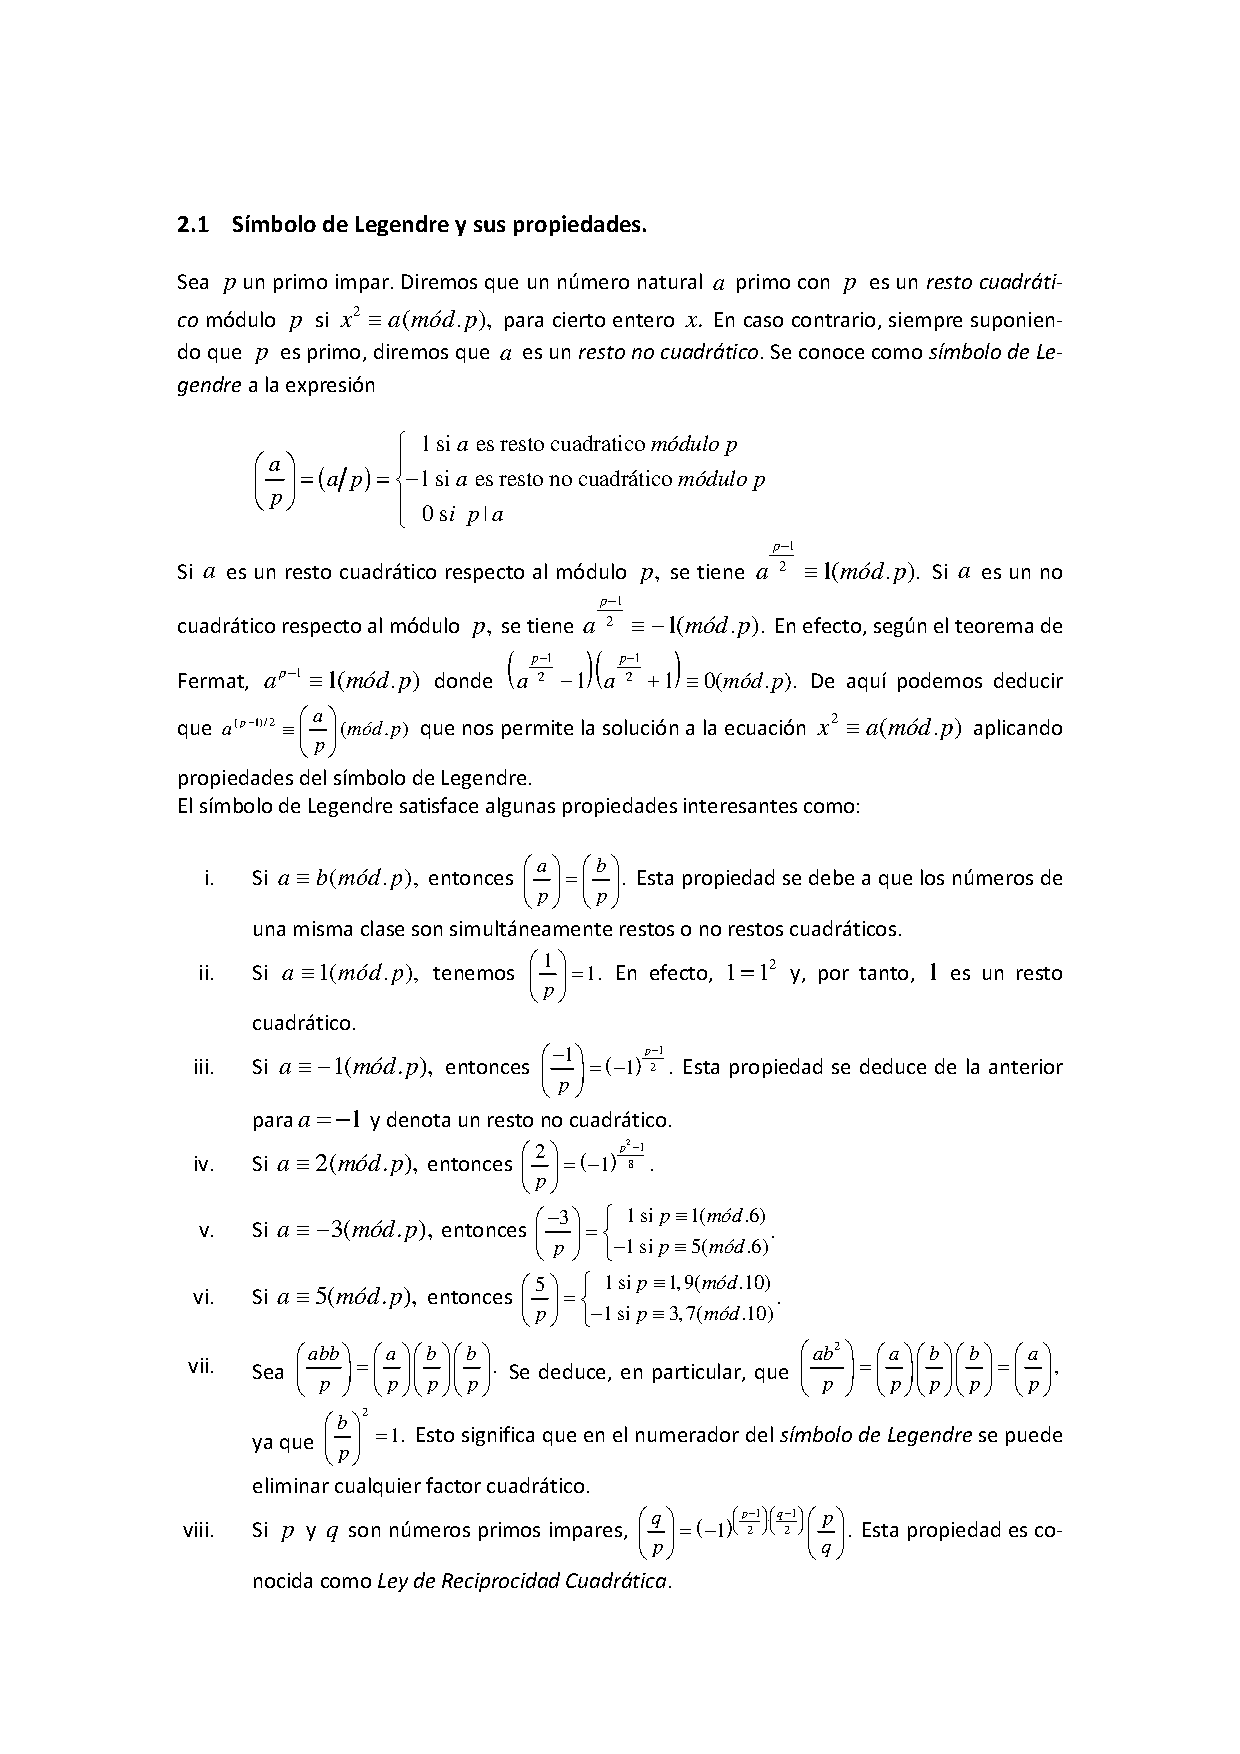
\includepdf[page={1-5}]{jacobi}

\chapter{ElGammal y el logaritmo discreto}

  \section{Generadores}

  \begin{figure}[h]
      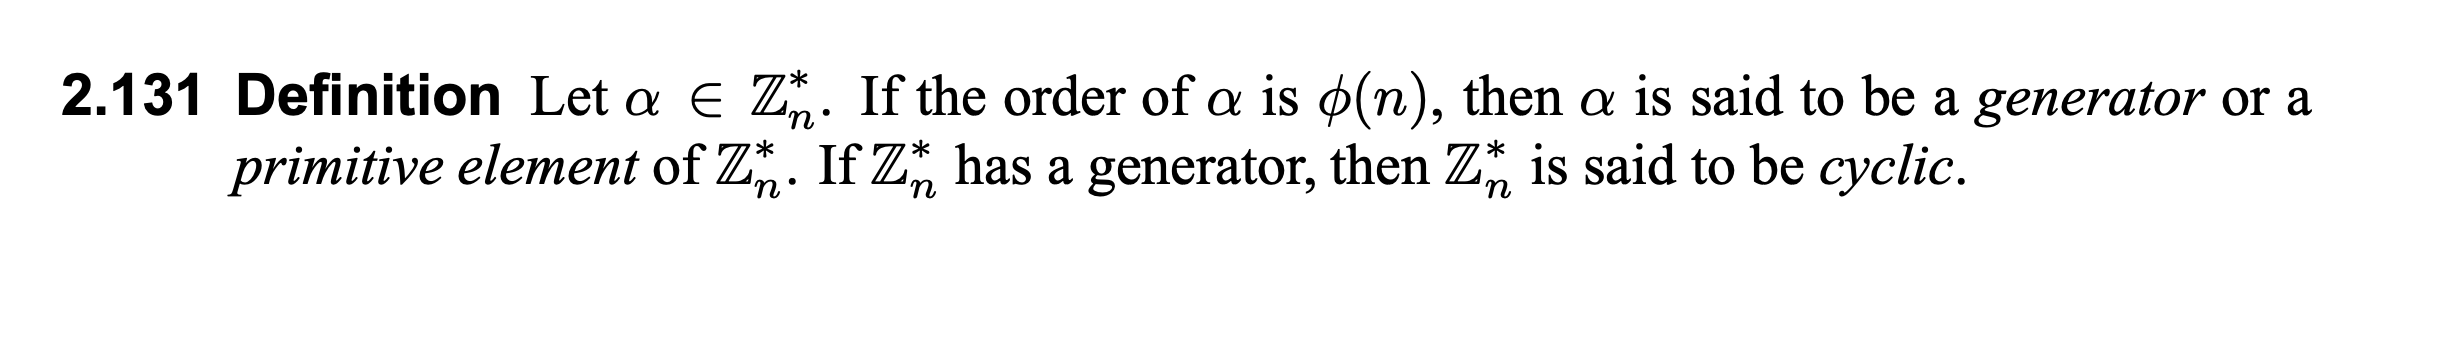
\includegraphics[width=\textwidth]{Gammal2}
      \caption{\cite{Menezes}}
  \end{figure}

  \begin{figure}[h]
    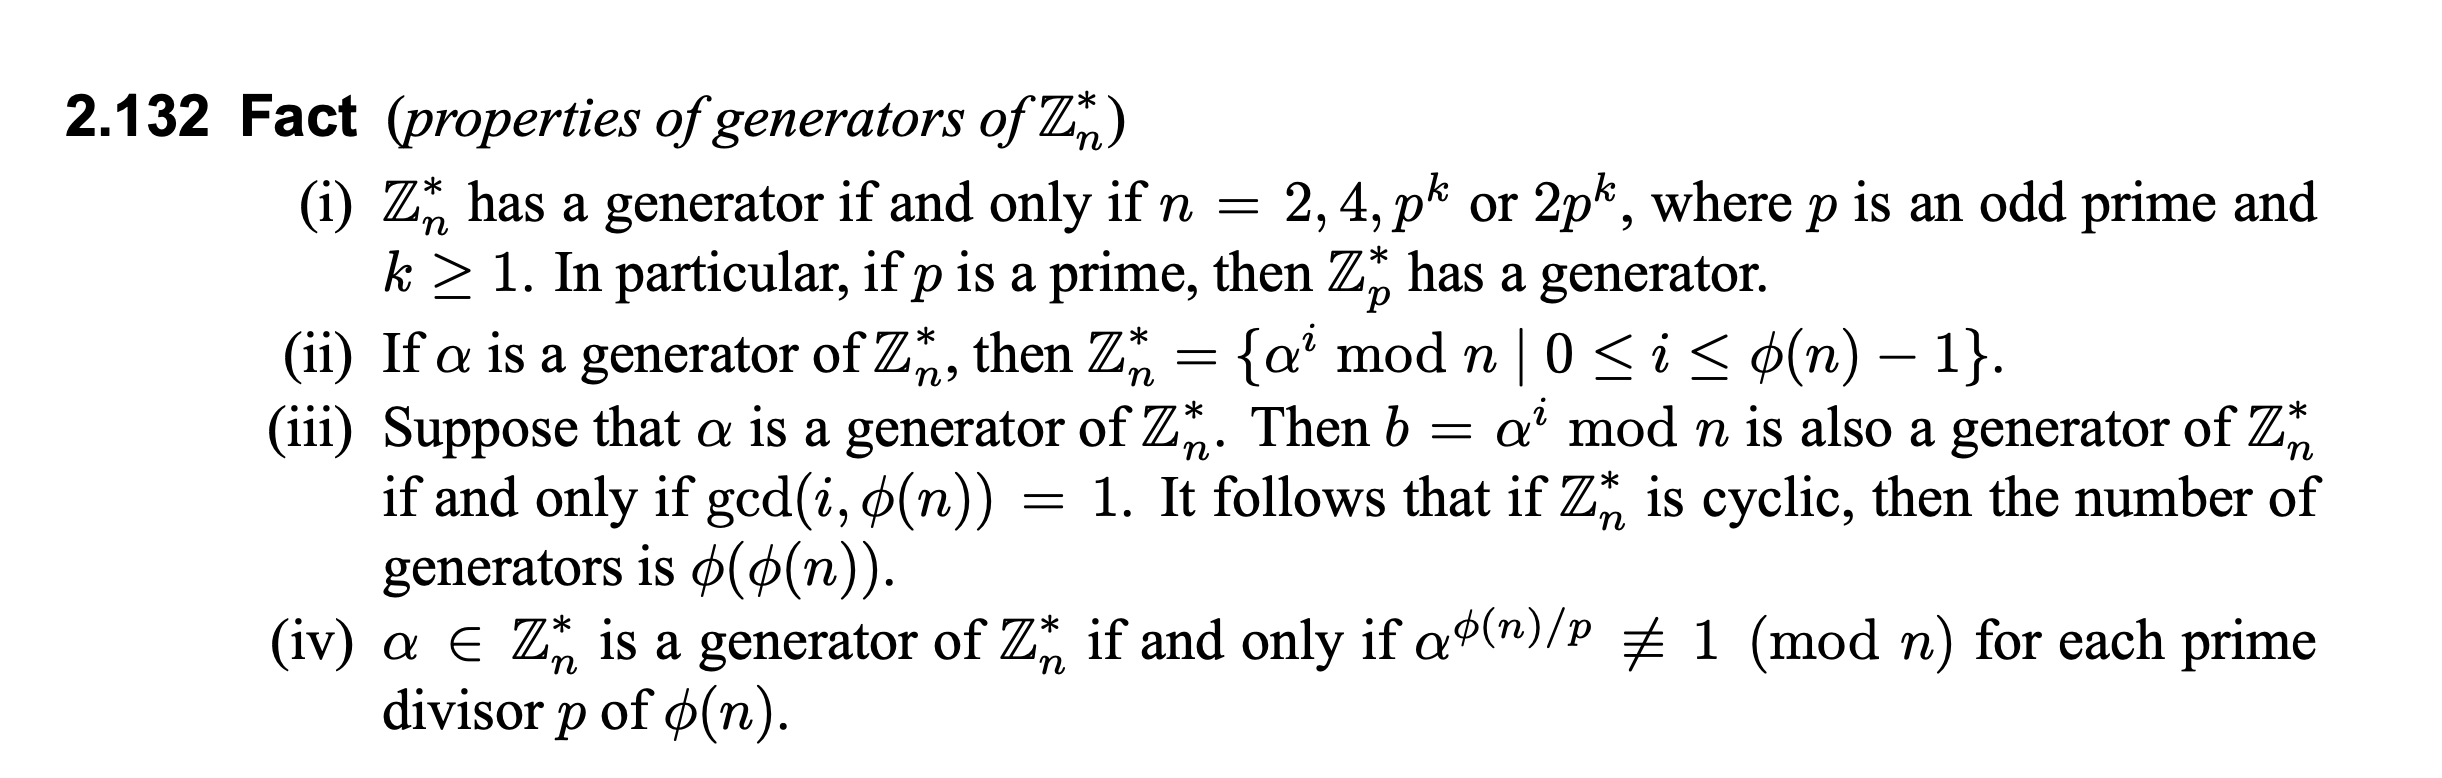
\includegraphics[width=\textwidth]{Gammal3}
    \caption{\cite{Menezes}}
  \end{figure}

    Primero que nada hay que probar que $2$ es un generador en $\Integers_{2027}^*$ 

    Para hacerlo (y por definición) podemos recordar que un generador es si el orden de $2$ sea igual a $\phi(n)$.

    Esto nos lleva a la definición de orden, que esta definido como la $t$ mas pequeña tal que $2^t \equiv 1 \mod{2027}$.


    Esto lo podemos probar con fuerza bruta, y un pequeño programa en Python:
    \begin{lstlisting}[language=Python, gobble=6]
      alpha = 2
      t = 1
      mod = 2027

      while pow(alpha, t, mod) != 1:
        t += 1
        
      print (t)
    \end{lstlisting}

    Llegando a que $t = 2026$ y dado que $2027$ es un primo es obvio que $\phi(p) = p -1 = 2027 - 1 = 2026$. 
    Por lo tanto la demostración por fuerza bruta esta lista.

    \subsection{Otra forma}

    Otra forma de llegar a esto es usando la idea del Menezes de que: $\alpha \in \Integers^*{n}$
    es un generador si y solo si $\alpha^{\frac{\phi(n)}{p}} \not \equiv 1 \mod{n}$ para cada
    factor primero de $\phi(n)$.

    Ahora como dijimos $\phi(p) = p -1 = 2027 - 1 = 2026 = 2 * 1013$, por lo tanto vamos a ir por sus factores primos:

    \begin{itemize}
      \item $2$
      
        Ahora vamos:
        \begin{MultiLineEquation*}{3}
          \alpha^{\frac{\phi(n)}{p}} 
            & \equiv  \alpha^{\frac{2026}{2}}  \pmod{2027}      \\
            & \equiv  \alpha^{1013}  \pmod{2027}                \\
            & \equiv  2^{1013}  \pmod{2027}                     \\
            & \equiv  2026  \pmod{2027}                         \\
        \end{MultiLineEquation*}

        Y mira no es uno, por lo que vamos bien.

      \item $1013$
      
        Ahora vamos:
        \begin{MultiLineEquation*}{3}
          \alpha^{\frac{\phi(n)}{p}} 
            & \equiv  \alpha^{\frac{2026}{1013}}  \pmod{2027}       \\
            & \equiv  \alpha^{2}  \pmod{2027}                       \\
            & \equiv  2^{2}  \pmod{2027}                            \\
            & \equiv  4  \pmod{2027}                                \\
        \end{MultiLineEquation*}

        Y mira no es uno, por lo que todo salio bien.

    \end{itemize}

    Por lo tanto $2$ es un generador. QED


  \clearpage
  \section{Calculo de indices}

    \begin{figure}[h]
      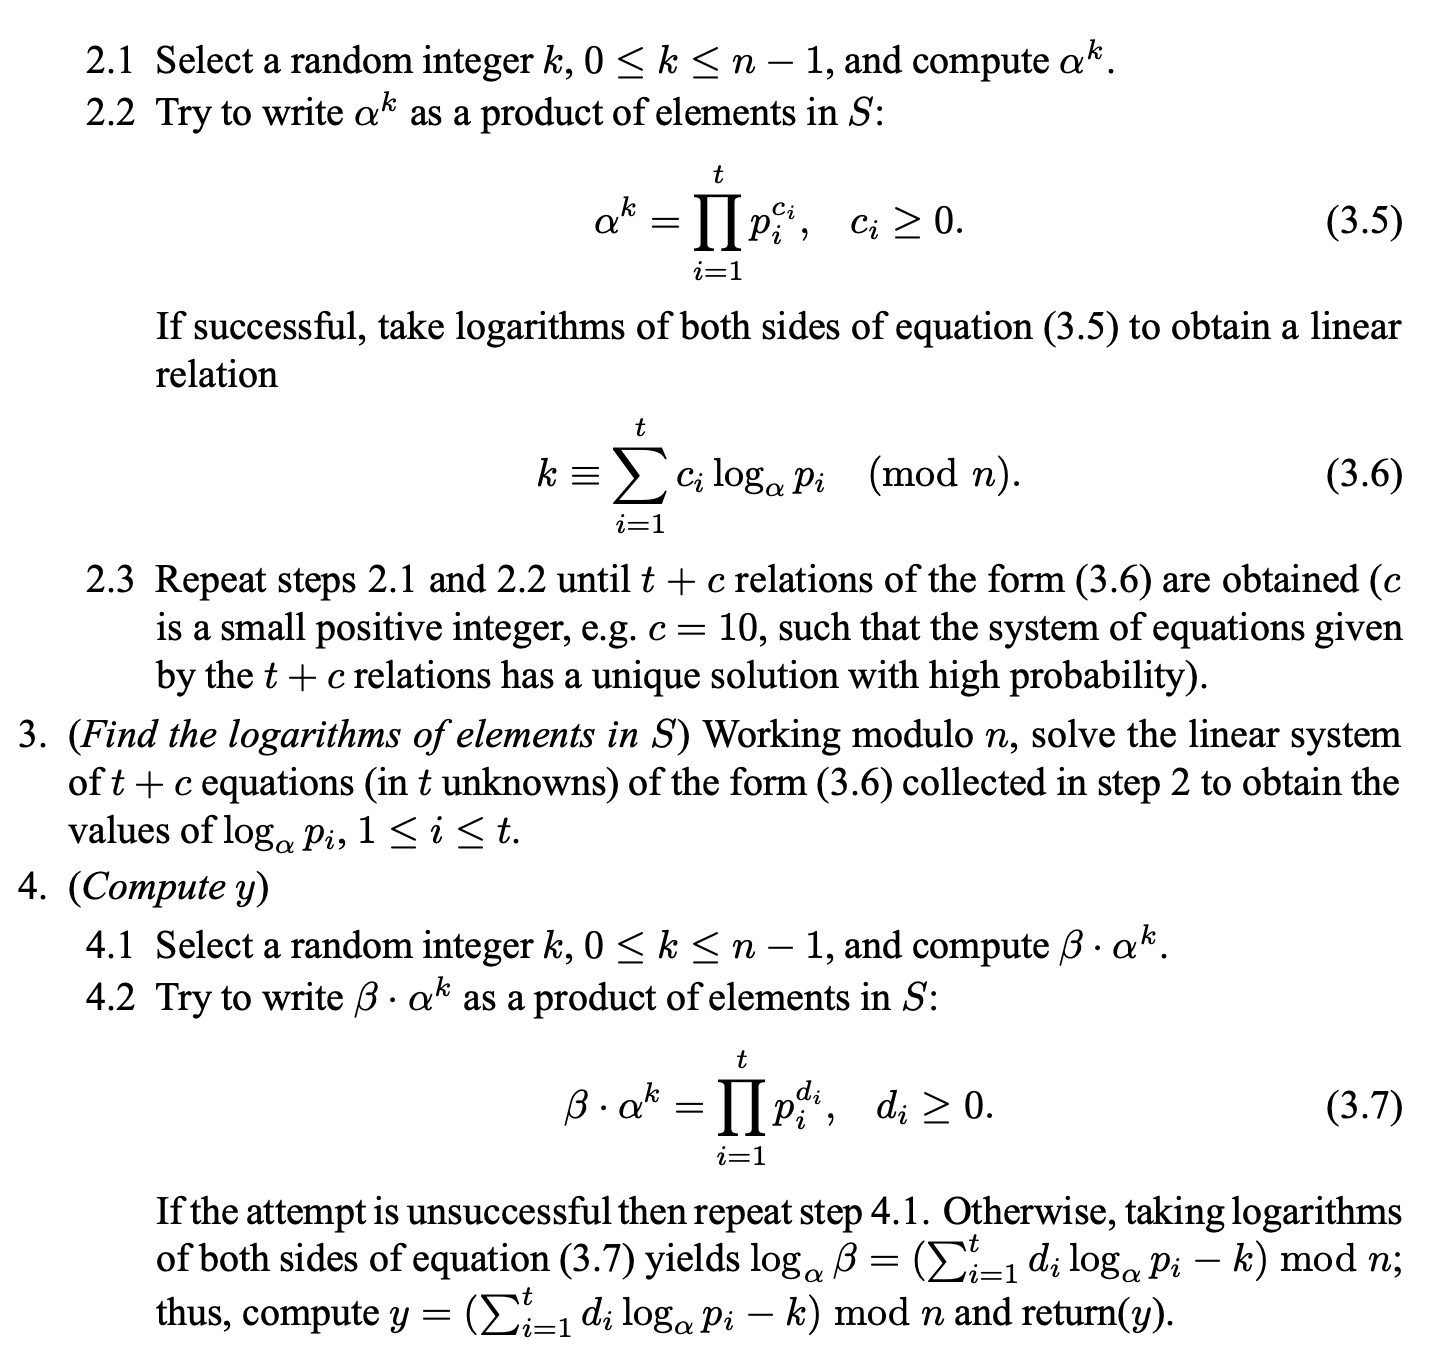
\includegraphics[width=\textwidth]{Gammal4}
      \caption{\cite{Menezes}}
    \end{figure}

    Ok, lo bueno es que ya me dieron la base: $2, 3, 5, 7, 11$.


    Ahora vamos a obtener 6 relaciones que fueron exitosas (dejo fuera las que fueron mal):
    \begin{itemize}
      \item $2^{769} \equiv 539 \equiv 11 * 7^2 \mod{2027}$
      \item $2^{1322} \equiv 231 \equiv 11 * 7 * 3 \mod{2027}$
      
      \item $2^{1912} \equiv 25 \equiv 5 * 5 \mod{2027}$
      \item $2^{1756} \equiv 14 \equiv 7 * 2 \mod{2027}$
       
      \item $2^{857} \equiv 567 \equiv 7 * 3^4 \mod{2027}$
      \item $2^{1799} \equiv 1250 \equiv 5^4 * 2 \mod{2027}$
    \end{itemize}

    Lo bueno es que hacer $2^x \mod{2027}$ es $O(log_2(n))$

    Con estas relaciones podemos escribir las siguiente ecuaciones:
    \begin{itemize}
      \item $769 \equiv log_2(11) + 2 log_2(7) \mod{2026}$
      \item $1322 \equiv log_2(7) + 2 log_2(3) \mod{2026}$
      
      \item $1912 \equiv 2log_2(5) \mod{2026}$
      \item $1756 \equiv 2log_2(7) \mod{2026}$

      \item $857 \equiv log_2(7) + 4log_2(3) \mod{2026}$
      \item $1799 \equiv 4log_2(5) + log_2(2) \mod{2026}$
    \end{itemize}

    Ahora, podemos ver esto como:
    \begin{itemize}
      \item $769 \equiv e + 2 d \mod{2026}$
      \item $1322 \equiv d + 2 b \mod{2026}$
      
      \item $1912 \equiv 2c \mod{2026}$
      \item $1756 \equiv 2d \mod{2026}$

      \item $857 \equiv d + 4b \mod{2026}$
      \item $1799 \equiv 4c + 1 \mod{2026}$
    \end{itemize}

    Ahora tras un poco de algebra bastante trivial podemos llegar a esto:
    \begin{itemize}
      \item $2, 3, 5, 7, 11$
      \item $log_2(2) \equiv 1 \mod{2026}$
      \item $log_2(3) \equiv 282 \mod{2026}$
      \item $log_2(5) \equiv 1969 \mod{2026}$
      \item $log_2(7) \equiv 1755 \mod{2026}$
      \item $log_2(11) \equiv 1311 \mod{2026}$
    \end{itemize}

    Ahora vamos a seleccionar enteros a lo random, despues de intentarlo un rato llegue
    a esto:

    $13 * 2^{1340} \equiv 550 \equiv 13 * 666 \equiv 550 \mod{2027}$
    y tenemos que $5^2 * 2 * 11 \equiv 550 \mod{2027}$

    Ahora si que podemos escribir que:

    \begin{MultiLineEquation*}{3}
      log_2(13) 
        & \equiv (2log_2(5) + log_2(2) + log_2(11) - 1340) \mod{2026}  \\
        & \equiv (2(1969) + 1 + 1311 - 1340) \mod{2026}                \\
        & \equiv 1884  \pmod{2026} 
    \end{MultiLineEquation*}

    Y podemos comprobar rápido que $2^{1884} \equiv 13 \mod{2027}$


    \clearpage
    \section{ElGammal}

      \begin{figure}[h]
        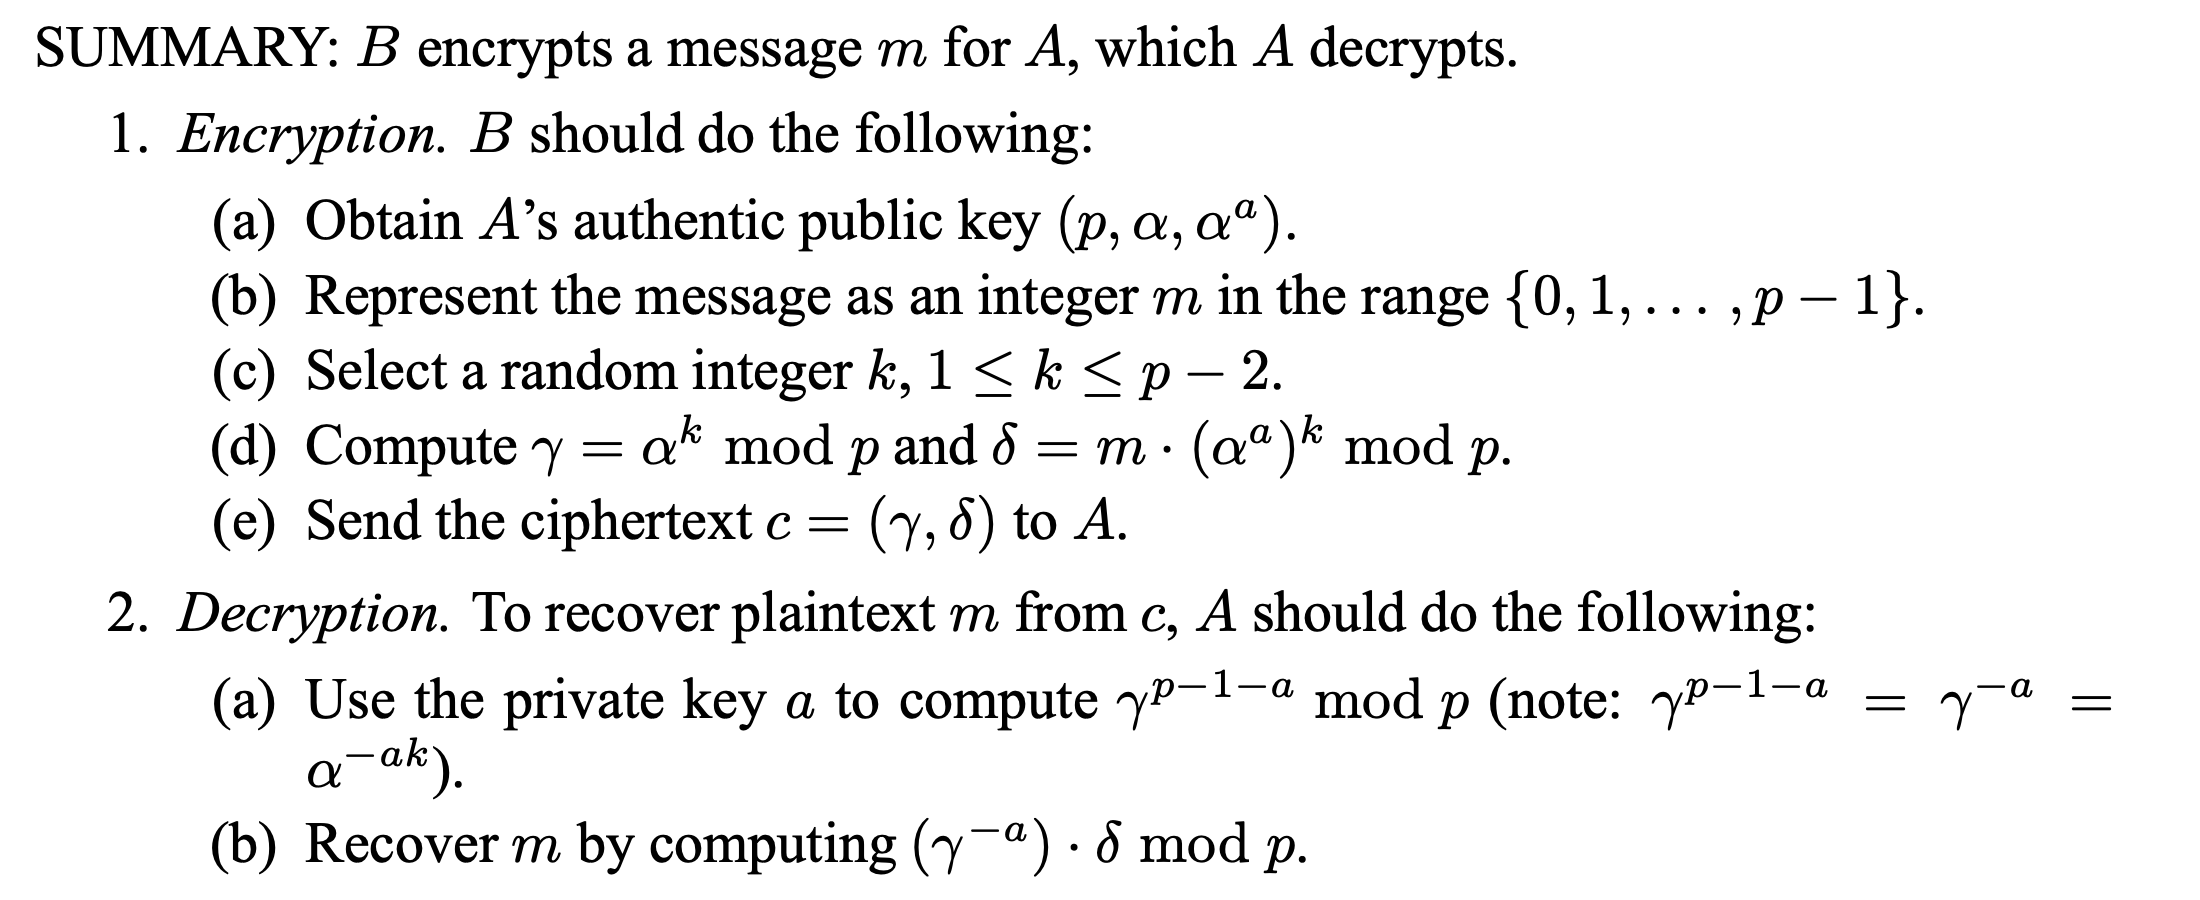
\includegraphics[width=\textwidth]{Gammal1}
        \caption{\cite{Menezes}}
      \end{figure}

      Ahora que tenemos la llave privada descifrar el mensaje es bastante sencillo, pero aun asi
      para que se entienda vamos por pasos:
      \begin{itemize}
        \item Por un lado lo que tenemos es una serie de pares por lo que podemos 
        imaginar que cifraron caracter por caracter, asi que vamos a solucionar un caracter y el
        resto será analogo.

        \item Ahora lo bueno es que justo el dia que escribo esto nos toco hacer ElGammal 
        en el laboratio por la idea esta muy fresca.

        Tu tienes un primo p ($2027$), eliges un generador ($2$), y un $2^k = 13$, estas son llaves
        publicas y justo la $k$ es la privada (ya vimos que es $1884$), ahora, dado un mensaje 
        $(y, \delta)$ para descrifrar lo que hacemos es $y^{p - 1 - a} * \delta \mod{p}$
        esto sale rapido:

        \item Por ejemplo para el primero mensaje tenemos que:
        \begin{MultiLineEquation*}{3}
          y^{p - 1 - a} * \delta \mod{p}
            & \equiv 128^{2027 - 1 - 1884} * 793  \mod{2027}  \\
            & \equiv 4  \pmod{2027} 
        \end{MultiLineEquation*}
        por lo tanto la primera letra del mensaje es una 'e'.

        \item Ahora vamos a simular el proceso que para algo somos computologos:
        \begin{lstlisting}[language=Python, gobble=10]
          mod = p = 2027
          a = 1884

          cipher = [
              (128, 793),   (128, 528),  (128, 1233),  (128, 793),
              (128, 793),  (128, 264),  (128, 793),  (128, 1850),
              (128, 1410),  (128, 1586),  (128, 1410),  (128, 1586),
              (128, 1762),  (128, 793),  (128, 528),
              (128, 1233),  (128, 87),  (128, 352),  (128, 1938),
              (128, 704),  (128, 1498),  (128, 87),
              (128, 1410),  (128, 1586),  (128, 1674),
              (128, 87),  (128, 1674),  (128, 1586),  (128, 176),
              (128, 1938),  (128, 87),  (128, 1674),  (128, 1145),
              (128, 1938),  (128, 793),  (128, 1674),
              (128, 87),    (128, 1233),  (128, 87),  (128, 1850),
              (128, 793),  (128, 87),
          ]


          def solve(y: int, delta:int) -> int:
              m = (pow(y, p - 1 - a, mod) * delta) % mod
              m = m % 26
              m += ord("a")  # works with ASCII

              return chr(m)


          message = "".join([solve(y, delta) for y, delta in cipher])
          print(message)
        \end{lstlisting}

        Dando el mensaje:
        \begin{lstlisting}[language=Python, gobble=10]
          esteejercicioestamuyfacilaligualquelatarea
        \end{lstlisting}

        Que buen mensaje.

      \end{itemize}

\chapter{Criba cuadratica y RSA}

  \section{Criba cuadratica}

    Primero que nada hay que seleccionar una base de factores, en este caso solo vamos a poner
    a los primos $p$ para los cuales $n$ es un residuo cuadratico modulo $p$:
    $S = Base = B = \Set{-1, 2, 3, 13, 17, 19, 29}$.

    Esto se hace con un sencillo programita:
    \begin{lstlisting}[language=Python, gobble=6]
      from sympy.ntheory import legendre_symbol

      def is_prime(n):
          if (n <= 1):
              return False
          if (n <= 3):
              return True

          if (n % 2 == 0 or n % 3 == 0):
              return False

          i = 5
          while (i * i <= n):
              if (n % i == 0 or n % (i + 2) == 0):
                  return False
              i = i + 6

          return True


      n = 87463
      for i in range(3, 50):
          if is_prime(i) and legendre_symbol(n, i) == 1:
              print(i)

    \end{lstlisting}


    Ahora lo siguiente es calcular $M = m = \Floor{\sqrt{n}}$, que en este caso $295$, finalmente
    vamos a calcular la tabla de la famosa criba cuadratica:

    \begin{tabular}{|c |c |c | c |c | c| }
      % And this is the name of all the headers
      \hline
      i & x & $b = q(x) = (x+m)^2 - n$ & factors & $a_i$ & $v_i$ \\ [0.5ex] 
      \hline\hline
     
      %Body
      1 & 1   & $(296)^2  - 87463 = 153$ & $3^2 * 17$                 & 296 & (0, 0, 0, 0, 1, 0, 0)    \\
      2 & 4   & $(299)^2  - 87463 = 1938$ & $2 * 3 * 17 * 19$         & 299 & (0, 1, 1, 0, 1, 1, 0)    \\
      3 & 12  & $(307)^2  - 87463 = 6786$ & $2 * 3^2 * 13 * 29$       & 307 & (0, 1, 0, 1, 0, 0, 1)    \\
      4 & -17 & $(278)^2  - 87463 = -10179$ & $-1 * 3^3 + 13 + 29$    & 278 & (1, 0, 1, 1, 0, 0, 1)    \\
      4 &  21 & $(316)^2  - 87463 = 12393$ & $3^6 * 17$               & 316 & (0, 0, 0, 0, 1, 0, 0)    \\
      5 & -30 & $(265)^2  - 87463 = -17238$ & $-1 * 2 * 3 * 13 * 17$  & 265 & (1, 1, 1, 1, 1, 0, 0)    \\
      \hline
    \end{tabular}

    Ahora, podriamos seguir haciendolo pero mira que ya tenemos que $a_1 + a_4 = 0$, asi que vamos a probarla:

    Ademas creo importante añadir que no hice estas cuentas solo a mano, llegue a hacer hasta 12 a mano, pero despues
    me di por vencido y mejor programe lo que estaba haciendo una y otra vez:
    \begin{lstlisting}[language=Python, gobble=6]
      from math import floor, sqrt
      from sympy import primefactors, factorint

      primes = [-1, 2, 3, 13, 17, 19, 29]
      n = 87463
      m = floor(sqrt(n))

      i = 1
      x = 1
      while (i <= 7):
          ai = x + m
          b = ai * ai - n

          factors = factorint(b, limit=29)
          if all([f <= primes[-1] for f in factors.keys()]) and len(factors) > 1:

              print(f"i={i} \t ai={ai} \t x={x} \t", end="")
              print(f"{b} = ", end="")
              for prime, exponent in factors.items():
                  print(f"{prime}^{exponent} * ", end="")
              print()

              i += 1

          x = -x + 1 if x < 0 else -x
      \end{lstlisting}

      Obteniendo esta tabla:
      \begin{lstlisting}[language=Python, gobble=6]
        i=1      ai=296    x=1    153     = 3^2 * 17^1 
        i=2      ai=299    x=4    1938    = 2^1 * 3^1 * 17^1 * 19^1 
        i=3      ai=307    x=12   6786    = 2^1 * 3^2 * 13^1 * 29^1 
        i=4      ai=278    x=-17  -10179  = 3^3 * 13^1 * 29^1 * -1^1 
        i=5      ai=316    x=21   12393   = 3^6 * 17^1 
        i=6      ai=265    x=-30  -17238  = 2^1 * 3^1 * 13^2 * 17^1 * -1^1 
        i=7      ai=347    x=52   32946   = 2^1 * 3^1 * 17^2 * 19^1 
      \end{lstlisting}


      Ahora, si, regresemos a lo que estabamos viendo, que $x = a_1 * a_4 = 296 * 316 = 6073 \mod{87463}$

      Ahora hagamos las $l's$:
      \begin{itemize}
      \item $l_1 = 0$
      \item $l_2 = 0$
      \item $l_3 = 4$
      \item $l_4 = 0$
      \item $l_5 = 1$
      \item $l_6 = 0$
      \item $l_7 = 0$
      \end{itemize}

      Con estos damos podemos ya calcular a: $y = 3^4 * 17 = 1377 \mod{87463}$.

      Ahora basta con sacar el $587 = gcd(6073 - 1377, 87463)$ 
      por lo que tenemos que $587$ es un factor no trivial, de hecho ya con este es obvio que:

      $87463 = 587 * 149$
    
  \clearpage
  \section{Ahora vamos con RSA}

    Ahora veamos que los parametros publicos son $(87463, 15157)$, es decir $(n, e)$
    y lo que estamos buscando es la llave privada (d) tal que $ed \equiv \mod{\phi(n)}$
    ahora sacar el inverso es sencillo si sabes la factorización de $n$, porque $n = p * q$, 
    entonces $\phi(n) = (p -1) * (q - 1) =  586 * 148 = 86728$, por lo que un simple algoritmo
    extendido de euclides nos da el inverso, dando que $d = 50485$.

    Con esta llave podemos descifrar todo muy sencillo:

    Es mas hice un programa que usando las ideas bases del algoritmo te ayuda con la pesada tarea de 
    descifrarlo uno a uno, despues de todo justo este fue un proyecto de laboratorio.

    \begin{lstlisting}[language=Python, gobble=6, basicstyle=\ttfamily\bfseries\scriptsize]
      from Crypto.Util.number import getPrime, GCD, inverse
      from math import log2

      big_length = int(log2(1e100))


      class RSA:
          def __init__(self):
              p = getPrime(big_length)
              q = getPrime(big_length)

              self.n = p * q

              phi_n = (p - 1) * (q - 1)
              public_key = phi_n - 2

              while GCD(phi_n, public_key) != 1:
                  public_key -= 1

              self.private_key = inverse(public_key, phi_n)
              self.public_key = public_key

          def get_keys(self):
              return self.n, public_key

          def encrypt(self, plaintext):
              return [pow(ord(char), self.public_key, self.n) for char in plaintext]

          def dencrypt(self, cipher):
              plain = [pow(char, self.private_key, self.n) % 26 for char in cipher]
              plain = [chr(m + ord("a")) for m in plain]

              return "".join(plain)


      solver = RSA()
      solver.n = 87463
      solver.private_key = 50485
      solver.public_key = 15157

      cipher = [
          21347, 41185, 31564, 41185, 76237, 73700, 53597, 21347, 31564, 73700,
          21347, 73700, 53597, 14144, 42561, 73700, 53597, 73593, 14420, 76237,
          41185, 76237, 23637, 14420, 1, 31564, 41185, 14420, 76237, 2136,
          41185, 22481, 21347, 73700, 73593, 14420, 76237, 73700, 53597, 82282,
          19930, 22481, 14420, 31564, 73700, 53597, 31564, 14420, 41185, 76237,
          14420, 53597, 82282, 73700, 14420, 53597, 53597, 19930, 67024, 14144,
          2136, 14144, 14420, 82282, 42561, 14420,
      ]

      message = solver.dencrypt(cipher)

      print(message)

      \end{lstlisting}

      Y llegamos a esto:
      \begin{lstlisting}[language=Python, gobble=8]
        paralospropositosdelalgebraelcampodelosnumerosrealesnoessuficiente
      \end{lstlisting}



\chapter{Generadores}

      Vamos a mostrar que el problema del logaritmo discreto no depende del generador.
      
      Sea $\alpha$ and $\gamma$ dos generadores de un grupo cíclico $G$ de orden $n$, y
      sea $\beta \in G$. 
      Sea $x = log_\alpha \beta$, $y = log_\gamma \beta$, y $z = log_\alpha \gamma$.

      Entonces $\alpha^x = \beta = \gamma^y = (\alpha^z)^y$.
      Por consiguiente $x = zy \mod{n}$, y 
      \begin{equation*}
        log_\gamma \beta = (log_\alpha \beta)(log_\alpha \gamma)^{-1} \mod{n}
      \end{equation*}

      Esto significa que cualquier algoritmo de que calcule logarítmos para una base 
      $\alpha$ puede ser usado para calcular logaritmos a cualquier otra base 
      $\gamma$ que también es un generador de $G$.

  \begin{thebibliography}{10}

    \bibitem{Menezes} 
        HANDBOOK of APPLIED CRYPTOGRAPHY 
        \textit{Alfred J. Menezes }. 

  \end{thebibliography}



\end{document}